\documentclass[a4paper]{article}

%% Language and font encodings
\usepackage[english]{babel}
\usepackage[utf8x]{inputenc}
\usepackage[T1]{fontenc}

%% Sets page size and margins
\usepackage[a4paper,top=3cm,bottom=2cm,left=3cm,right=3cm,marginparwidth=1.75cm]{geometry}

%% Useful packages
\usepackage{amsmath}
\usepackage{graphicx}
\usepackage[colorinlistoftodos]{todonotes}
\usepackage[colorlinks=true, allcolors=blue]{hyperref}

\title{Assignment 7: ZombieApocalypsePrep-SIS}
\author{Christa Wright (wrighch3),\\ Kuan-Yu Lai(laik),\\ Blake Hudson(hudsonbl), \\Eric Sisson (sissone), \\ Jorge Guzman Nader(guzmannj)}

\begin{document}
\maketitle

\includegraphics[width=\textwidth]{zombie.jpg}
\pagebreak
\tableofcontents
\pagebreak

\section{Product Release}
The user will run the software by accessing the website. Upon reaching the home page, the user
will find several options. The options are located in the navigation bar. User stories
1-12 describe how the user will interact with the website. The navigation bar is where the buttons
for accessing different features of our website are located. Which those features are described by
the user stories. To go into more depth in how the user will access each of these stories or features,
is simple user input upon clicking targeted features. A run through of how the system will be used is
discussed by the following steps:
\newline
\newline
The instructions for using the software ere:
\newline
\newline
1.Open the url with any web browser( we have tested the webpage in firefox, chrome and Internet explorer).
\newline
\newline
2. In the home page you create a new goal, navigate to the history of previously created goals, go to the nutrition page, or go to the contact us tab and check the level bar that shows user progress.
\newline
\newline
3.In the create new goal button the user can insert an activity and a time for or repetition set to consider the activity complete, ex.the user input run in the activity bar and 10 miles in the distance and time bar the click "make a new goal".
\newline
\newline
4.When the user click in the history part the web page will show the previously made goals and the date they were made.
\newline
\newline
5. When the user click in the nutrition button, the user will be able to enter weight, height, gender and age, based in this info the software will give a table with the recommended caloric intake, and micro/macro nutrients that this user must consume based in medical and biochemical data. 
\newline
\newline
6. Every time that the user finishes a goal experience point will be awarded that will allow the user to increase level.
\newline
\newline
7. The web page is mobile friendly and can be access anywhere when Internet connection is present.
\newline
\newline

\section{User story}
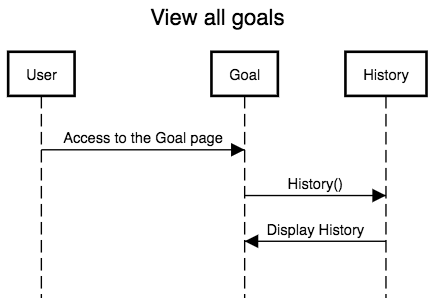
\includegraphics[width=\textwidth]{view_goals.png} 
\newline
\newline
\newline
\begin{itemize}
  \item Christa worked in this feature 
  \item We used 1 laptop to complete the task
  \item The task required approximately 3 days(around 10hrs).
  \item The current status is implemented and with some testing.
  \item More testing needs to be completed, the progress bar and points per goal needs to be tested.
  \item Yes, the diagram is useful since it helps us understand the relation between each feature.
  \item Currently we feel like the diagrams are good for us.
\end{itemize}

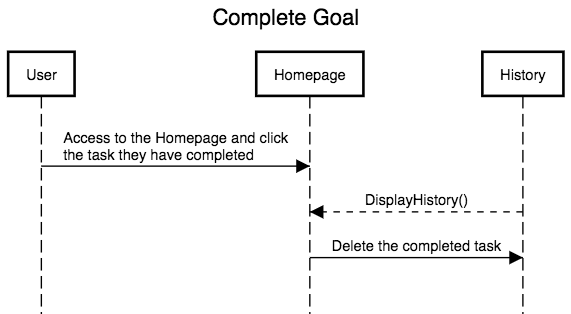
\includegraphics[width=\textwidth]{complete_goal.png} 
\newline
\newline
\newline
\begin{itemize}
	\item Christa and York was working on this feature. 
	\item A pair of laptops was used for this.
    \item The implementation of this feature took approximately 1 day.
    \item The current status is implemented.
  \item This feature still needs to be tested intensively 
  \item Yes, the diagrams were useful and helped us to filter the actual needs of the software development process
  \item The diagrams were fine as they are.
\end{itemize}

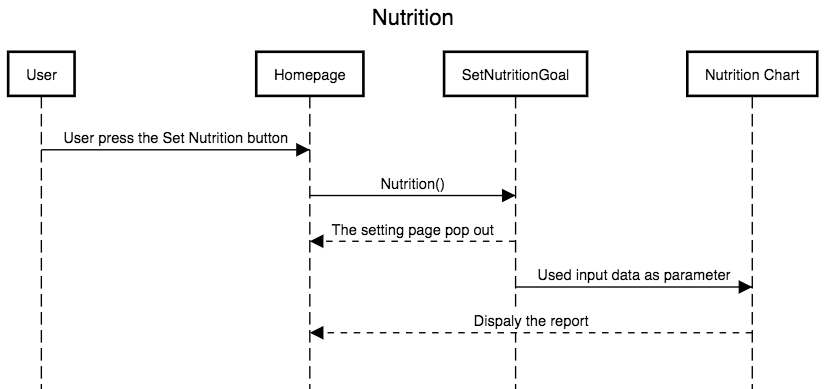
\includegraphics[width=\textwidth, height=8 cm]{nutrition.png}
\begin{itemize}
	\item Jorge and Christa worked in this feature. 
	\item We used separated laptops to work on this
    \item The task took around 2 days(8 hrs)
    \item The current status is implemented and tested 
  \item We need to implement the micro/micro nutrients diagrams.
  \item Yes, the diagram was useful, because allow us to conceptualize better the ideas to be implemented.
  \item We did not need more diagrams
\end{itemize}

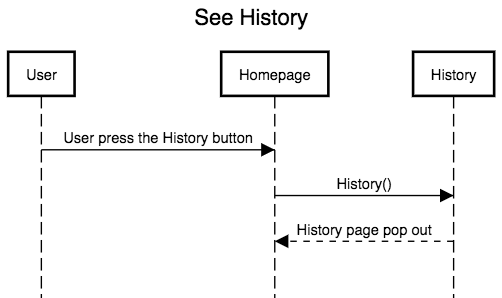
\includegraphics[width=\textwidth, height=8 cm]{see_history.png}
\newline
\begin{itemize}
	\item York and Christa are working on this feature. 
	\item We used different different laptops for this part.
    \item This task took around 5hrs.
    \item The status of this feature is implemented.
  \item The functionality of the page.
  \item We still need to test this functionality. 
  \item Yes, the diagram is useful because helped us to organize out work better.
  \item We wished we had more database diagrams, but we figure out a solution around this.
\end{itemize}
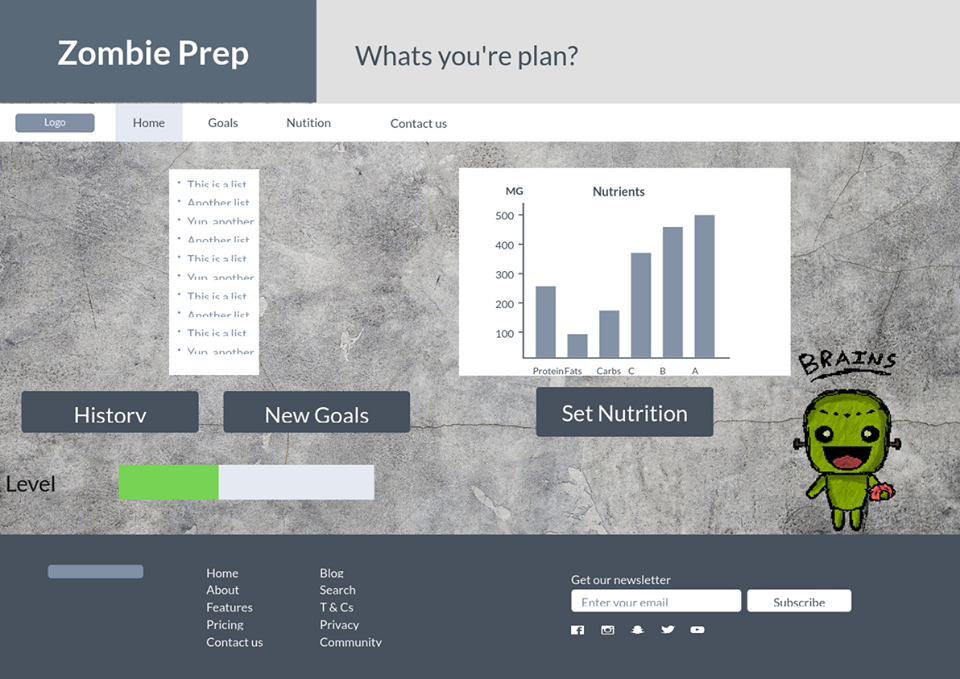
\includegraphics[width=\textwidth, height=8 cm]{page.png}
\newline
\begin{itemize}
	\item Eric and Christa are helping in this feature. 
	\item We worked in separate laptops while talking with each other.
    \item The task took around 4hrs
    \item The current status is implemented.
  \item We still need to test this feature and link the level bar to the goals that awards points.
  \item We did not have an explicit diagram for this feature.
\end{itemize}
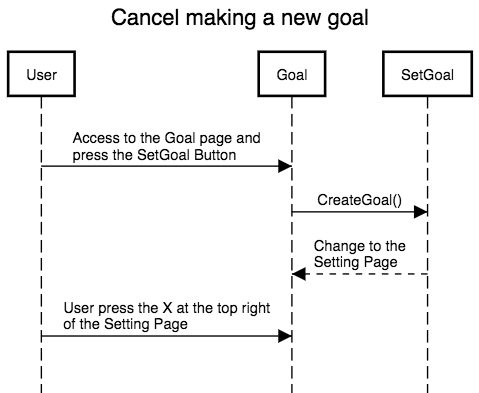
\includegraphics[width=\textwidth]{cancel_goal.png}
\begin{itemize}
	\item York worked on this feature. 
	\item Just one laptop was used in this feature
    \item The implementation took 2hrs
    \item The current status is implemented and tested.
  \item No extra functionalities are needed for this feature.
  \item Yes, the diagrams were useful because helped us focus in the required steps for finishing the code.
  \item We did not required further diagrams for this feature.
\end{itemize}
\section{Design changes and rationale}
The customers have been easy to get a hold of and respond quickly to questions. They provide insightful information on how the Zombie Prep App should look, and offer ideas on how to implement it. 
\newline
\newline
We asked the customers about the hosting of the web application and  plausible options for  implementing our server. The customer agreed in hosting the web application in the school server because the students working on the project have access to it, and is easier to deploy. The costumer also inquiry about how the home page would look and asked that the results for the nutrition and goals will be displayed in the home page.
\newline
\newline
The customer also suggested making the web page accessible to make it easier for people who are colorblind or who are visually impaired, such as not seeing well. Due to HTML having pre - built functionality already in it, the group won't have to put in much more effort to make the web application accessible to users. 
\newline
\newline
The bootstrap that the page already uses will also make it accessible when the page is zoomed in. The user would be able to tab through links easily with the HTML that the page uses, and will be able to tab between the forums as they enter information into it. 
\newline
\newline
The user stories that we changed were:
\newline
\newline
The main goals page got a different look with the input bars, tabs and colors being different that from the original design, the database got changed to the engineering servers and now holds the history for goals created and manage accounts.
\newline
\newline
Most of the code functionalities got changed to php so it worked better with our new interface, and the server, also php have good sanitation functionalities that helped in our development process,The scroll bar that the program had before got changed to allow the user to enter custom input that will be validated by a test software.
\newline
\newline
History got implemented in the new server in a different way that was implemented before, the nutrition page got extra functionalities such as display calories in a different graphical format, and now it uses imperial system instead of metric for calculations.
\newline
\newline
Finally we used mysql for the database and changed the css to be more compact and easy to modify by the contributors.
\newline
\newline
\newline
\newline

\section{Refactoring}
The way we re-factored our code is through including php files embedded in our html code.
\newline
\newline
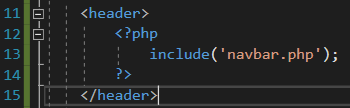
\includegraphics[width=\textwidth]{codeSnippet.PNG}
\newline
\newline
As you can see in the image above, the header includes a php file which contains the html code used for the navigation bar on our website. This makes reading the code easier by decrementing the amount of code given on a given page. This is similar to the Making Dealing with generalization. Where we collapse the hierarchy of the code into php snippets. This way when the user calls different pages; since my group has developed the pages to look similar, we re-use the html code for each page.
\newline
\newline
Including php snippets is similar to using methods in object oriented programming languages. Where we just include the php for wherever structurally we need to re-use html code. Overall this immensely makes code easier to read. This is because you can now select a file(method) containing html code for each section of our website.
\newline
\newline
The following list are php files that contain html code snippets:
\begin{enumerate}
\item add\_new\_goals.php
\item calc.php
\item connect\_sql.php
\item goals.php
\item head.php
\item index.php
\item navbar.php
\item new\_goal.php
\item nutrition.php
\item set\_nutrition.php
\end{enumerate}

\noindent The main php file which contains the bulk of our code for our pages is index.php. add\_new\_goals.php, goals.php, nutrition.php redirect the user to new pages with similar url path names as the php methods. Other related refactoring methods would be organizing data in our database. We are using the onid database system specifically jQuery. That is where we create our input fields for the user input. Then in the systems code, it can reference the specified SQL column entries. This method 

\section{Tests}
Our unit testing involves testing multiple individual units at once to expedite testing. The approach our software is accepting tested units is by instantiating static variables for instances of user input. This way we can manually test parameters to throw errors. 
\newline
\newline
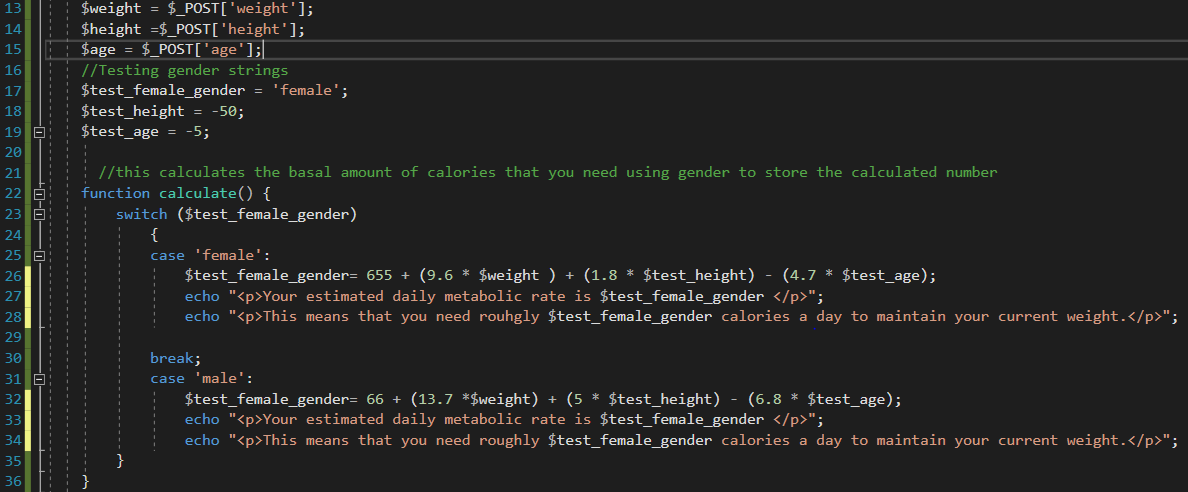
\includegraphics[width=\textwidth]{test1.PNG}
\newline
\newline
The figure above shows a snippet of unit test code for our add nutrition feature. The variables named with test\_ are the renamed variables that in our production code will read user input. But, in the case of our unit testing, we set the values to constants. This way during compilation we see if the variable is accepted by the system. In this test, we are identifying if a variable is negative or non-numerical. We also test the sex that the user will input. In this test, we use female as the sex, testing the correct switch statement, and negative values, testing the height and age.
\newline
\newline
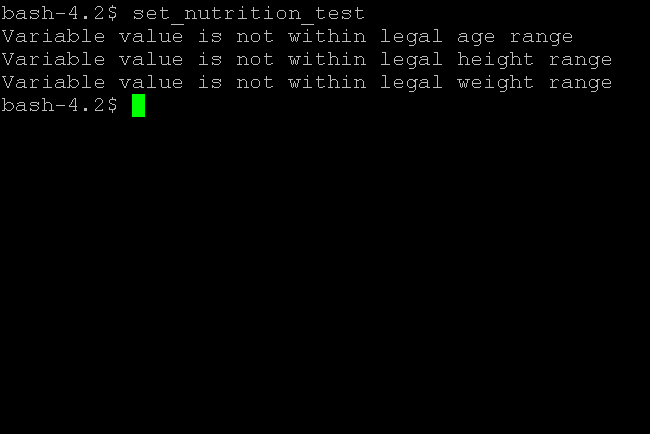
\includegraphics[width=\textwidth]{test5.PNG}
\newline
\newline
As shown in the image above, our test failed. This test was successful in proceeding with our new approach. Our new approach will modify the current code in the php, and add variable checking features. Specifically, for numerical values we will set an integer range using php's validation features. FILTER\_VALIDATE\_INT is the flag we must set for checking a numerical range. Since the string field for the sex is not text entered in by the user, we aren't testing the validity of the characters itself, we are only testing whether the case statement branched correctly.
\newline
\newline
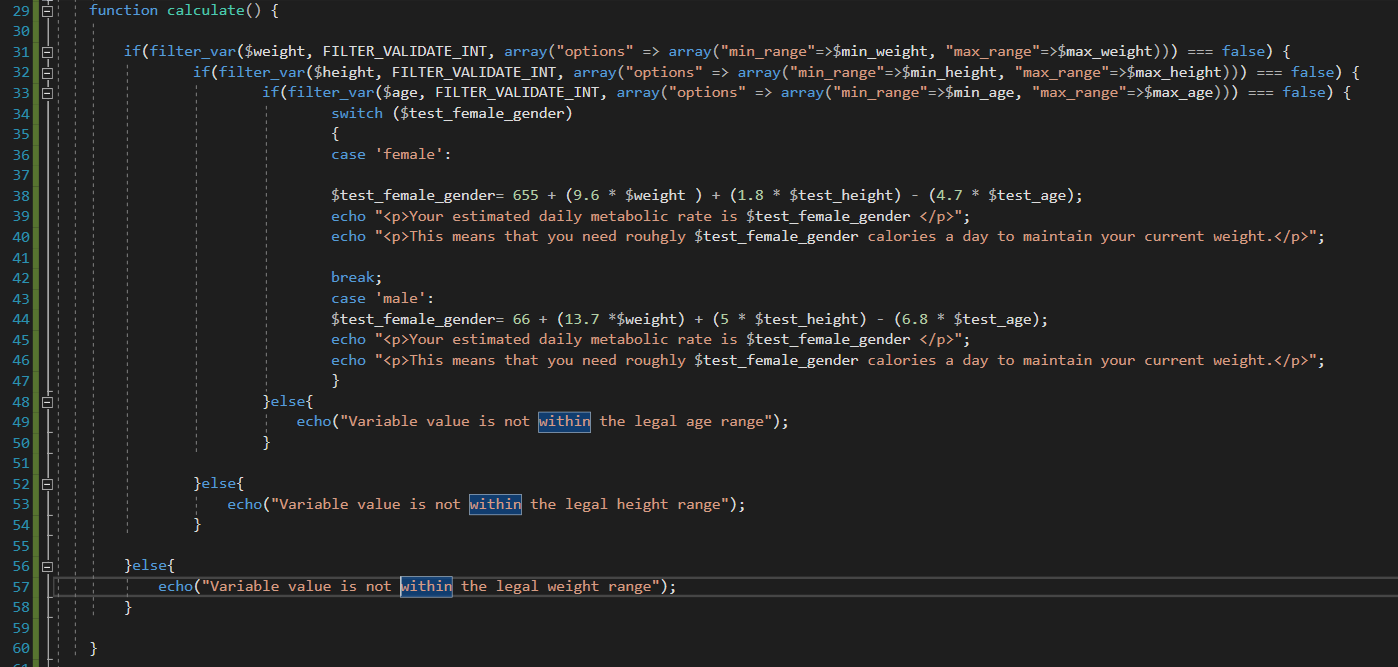
\includegraphics[width=\textwidth]{test7.PNG}
\newline
\newline
The image above fixes our initial test results. If the height, age, or weight is invalid, a print statement will be printed if so and the system will not accept the input. Although from the users prospective the invalid input would appear to process because it will redirect the user to the same page which is what occurs when valid input is gathered. The catch is that no data is saved into the data base when an invalid flag is caught. So in all, the invalid input is dismissed without changing any saved data. It's a simple way of handling invalid input. 
\newline
\newline
The next unit test will test the add goal feature in our software. Add goal is our core feature in our system. The units we are testing are two inputs provided by the user. The first unit is a character string. The string can be any string entered into the system. The purpose of this is for the user to create completely dynamic workouts with set interval integer goals provided in the second input unit. The test itself for the first input unit will be if the string is a string and not a integer. The second input unit will check if the integer is positive and between a range of 0 to 10000. 
\newline
\newline
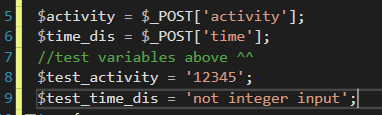
\includegraphics[width=\textwidth]{test3.PNG}
\newline
\newline
The image above shows the code provided for testing the user input. We statically embedded values that would throw an error in the code. This style of testing is Unit Testing. The string parameter is given an integer, the int parameter is given a string. This will test the integrity of our system. 
\newline
\newline
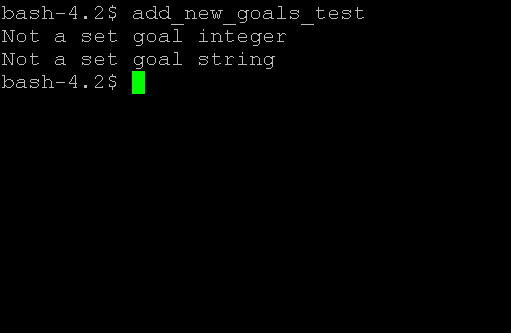
\includegraphics[width=\textwidth]{test6.PNG}
\newline
\newline
As seen above the code failed. Which is completely expected. The code will be modified to catch those results. Similarly to how the first test was resolved. 
\newline
\newline
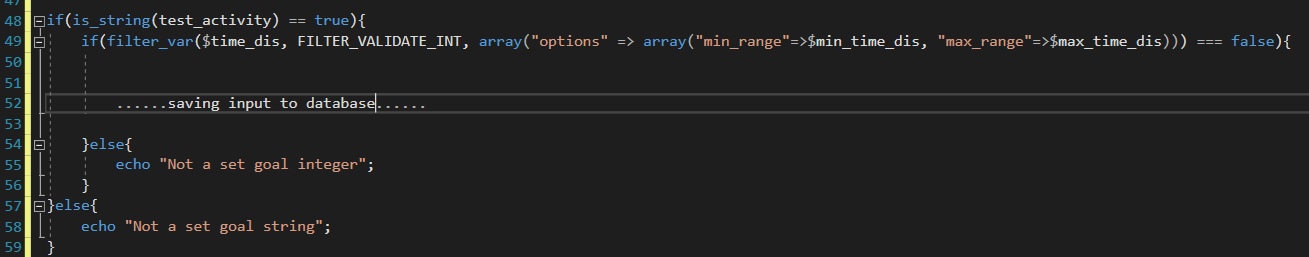
\includegraphics[width=\textwidth]{test4.PNG}
\newline
\newline
The conditionals in the code above is semi sudo code for the actual implementation. The code validates the users input. Again, the data will not be saved if the user enters invalid input. Instead the user will be rerouted to the main screen as if the user entered in data similar to if the user inputed valid data. 

\section{Meeting report}
This week we meet to finish most of our user stories and work in the code for the presentation next week.
\begin{itemize}
\item New schedule: 
\newline
\newline
Adding goals will be done this 03/10/2018
\newline
The database interactions will be ideally done 03/13/2018
\newline
History will be done this 03/11/2018
\newline
Progress bar and experience points will be done this 03/13/2018
\newline
Testing for different functionalities will be done this 03/11/2018
\newline
Add new functionalities to the nutrition feature and a display bar will be done this 03/12/2018
\newline
CSS polishing will be done this 03/13/2018
\item Progress this week: 
\newline
\newline
implemented the database, we add the nutrition calculation features, we improve the User Interface, we add a progress var for the leveling up in the web page, we wrote some unit and system test for our application, we implement the add goal and cancel goal features and we made our web page portable friendly. 
\item Plans and goals for next week: 
\newline
\newline
For next week we plan to implement a fully functional experience bar that is linked to the points system that our goals uses.
We also plan to to display the nutrition information in the main page in the form of a bar graph. Another functionality that we want to implement is a fully supported history menu in the database that work will all the other functionalities in the page.
\item Teammate contribution:
\newline
\newline
York contributed with the canceling goals feature and the history feature.
\newline
\newline
Christa made the main skeleton for all the pages, the user interface, the database,the goal creation and helped in most of the features being implemented.
\newline
\newline
Jorge made the nutrition page and calculations, he also wrote the documentation and charts for the web page, additionally he contributed to the set up of the git hub paths and validation.
\newline
\newline
Blake contributed to the documentation, and made the testing for the web page.
\newline 
\newline
Eric made the progress bar in the web page.
\item Costumer meeting 
Our costumers not just meet with us but also contributed in great part to the development of the web page, both by writing code and by planning how to implement the page.
\item The costumers were reasonable in their suggestions and helped to diminish the feature creep effect. The php migration was one of the most challenging steps in the overall development process do to the learning curve that it requires, but thanks the the costumers diligence and the attention of every team member, we successfully circumvent this obstacle.   
\end{itemize}

\pagebreak




\end{document}